\noindent
\includegraphics[height=1.25cm]{images/pictograms/replication}
\includegraphics[height=1.25cm]{images/pictograms/FEM}
\includegraphics[height=1.25cm]{images/pictograms/temperature}
\includegraphics[height=1.25cm]{images/pictograms/nonlinear}
\includegraphics[height=1.25cm]{images/pictograms/paraview}

%%%%%%%%%%%%%%%%%%%%%%%%%%%%%%%%%%%%%%%%%%%%%%%%%%%%%%%%%%%%%%%%%%%%%%%%%%%%%%%%%%%%%%%%%%%%%%%%%%%

\begin{flushright} {\tiny {\color{gray} python\_codes/fieldstone\_178/text.tex}} \end{flushright}

%\lstinputlisting[language=bash,basicstyle=\small]{python_codes/template_keywords.key}

\par\noindent\rule{\textwidth}{0.4pt}

\begin{center}
\inpython
{\small Code: \url{https://github.com/cedrict/fieldstone/tree/master/python_codes/fieldstone_178}}
\end{center}

\par\noindent\rule{\textwidth}{0.4pt}

Last revision: August 11th, 2025.

\par\noindent\rule{\textwidth}{0.4pt}

%%%%%%%%%%%%%%%%%%%%%%%%%%%%%%%%%%%%%%%%%%%%%%%%%%%%%%%%%%%%%%%%%%%%%%%%%%%%%%%%%%%%%%%%%%%%%%%%%%%

{\color{red} \large This was once used for teaching purposes at the UU and then retired.}

%%%%%%%%%%%%%%%%%%%%%%%
\section*{Geological Context}

The formation of a new ocean during plate tectonics requires stretching, thinning and breakup of a 
continental plate into two or more fragments. The deformation of the lithosphere during continental 
rifting leads to mantle upwelling, which at some point generates melt by mantle decompression creating 
a new oceanic crust. The investigation of the crust and lithosphere deformation during continental 
rifting is possible via geological and geophysical observations, and by using different model approaches.

Understanding extensional processes on the real Earth primarily and indubitably relies on the studies of 
past or currently-active regions under extension. Those regions includes any simple sedimentary basins, 
active or aborted rift systems, present-day continental rifted margins or fossil analogues margins exposed 
in orogens. The types of observations are diverse including field-geology observations, seismic imaging, 
tomography and much more. All those data require interpretation and explanation which lead to new concepts and generation of models. 

%----------------------------
\subsection*{Conceptual models}

Conceptual models are more or less elaborate cartoons based on geological and geophysical observations. 
They help to visualize concepts in a simple manner and they can be considered as the first step in understanding 
lithosphere deformation. For example, the concept of pure shear (\cite{mcke78}) and simple shear (\cite{webu86}), 
as shown in the figure below are two important contributions to explain associated rift and margin 
geometries during lithosphere extension. \cite{fort81}

\begin{center}
\centering
\includegraphics[width=10cm]{python_codes/fieldstone_178/images/Lfig1.jpg}\\
{\captionfont End-member styles of rifting; symmetric, asymmetric and compound (\cite{lies86}) narrow models, 
and the wide rift mode. (from \cite{hube07})}
\label{conceptModel}
\end{center}

%-------------------------------
\subsection*{Analogue models}

Analogue modelling is performed in laboratories and uses different types of materials to reproduce and simulate 
features of crustal and lithosphere deformation (see for instance Fig. (\ref{analogModel})). While analogue models 
are simple, intuitive and good for 3D, they cannot take into account a complicated rheological evolution. 

\begin{center}
\includegraphics[width=9cm]{python_codes/fieldstone_178/images/Lfig2.jpg}\\
{\captionfont Evolution of a 4-layer experiment containing 3-layer weakness zone for comparison with 
the East African Rift System. (from \cite{cort12})}
\label{analogModel}
\end{center}

%-----------------------------
\subsection*{Numerical models}

Numerical modelling is a necessary tool for geodynamics since tectonic processes are too slow and too deep in the Earth to be observed directly. Since the 1980s, numerical geodynamic modelling has been developing very rapidly in terms of both the number of various applications and numerical techniques explored. Many geodynamic problems can be described by mathematical models, i.e. by a set of partial differential equations and boundary and/or initial conditions defined in a specific domain. Numerical models are based on the general physical-mechanical principles (e.g., momentum, thermal, and mass conservation equations) and predict what would happen when the crust and mantle deform slowly over geological time. The equations involved can be solved with a specific numerical method (e.g., Finite Difference Method, Finite Element Method, etc). 

When looking at a specific geological problem, one first needs to design an initial model with certain boundary conditions. Then the model can be simulated by running a computer code, which produces the time-dependent evolution of the model. 

Two types of numerical modelling approaches can be discriminated: kinematic and dynamic approaches. 

In kinematic models, the crust and lithosphere deformation is prescribed by a flow velocity field. The flow field can be an analytical solution (e.g., pure shear deformation mode of \cite{mcke78}), or coming from a numerical solution \cite{jekm16}. This allows the advection of temperature and material and thereby the total control of the resulting deformation. Although kinematic models omit rheological properties and the physics of its evolution, their simplicity of use allows quantitative calibration on natural case laboratories. Kinematic models can be applied to predict e.g., subsidence, heat-flow or the architecture of sedimentary basins and rifted margins. In \cite{jekm16}, a kinematic model was developed to determine the full deformation history of the Iberia-Newfoundland rifted margins formation: 

\begin{center}
\includegraphics[width=10cm]{python_codes/fieldstone_178/images/Lfig3.jpg}\\
{\captionfont Application of a kinematic model of lithosphere deformation to the Iberia-Newfoundland rifted margins formation (from \cite{jekm16})}
\label{KinemModel}
\end{center}

In dynamic models as shown in the figure below, the mode of lithosphere deformation is defined by 
constitutive equations where the rheology is fully thermo-mechanically coupled (\cite{thie11}), and thus often showcases
nonlinear couplings: heat transport (e.g. thermal convection), phase changes, complex rheology (e.g. non-Newtonian 
flow, strain softening, elasticity and plasticity - \cite{hube03,hubb05,hube07}), melting and melt 
migration (\cite{arhm09, latb17}), chemical reactions, solid body motion, lateral forces, etc. 

\begin{center}
\includegraphics[width=8cm]{python_codes/fieldstone_178/images/Lfig4.jpg}\\
{\captionfont Example of a dynamic model setup (\cite{hube03})}
\label{DynamModel}
\end{center}


Lithosphere and asthenosphere deformation is usually initiated using initial anomalies implanted within the 
lithosphere\footnote{http://blogs.egu.eu/divisions/gd/2017/10/18/planting-seeds-of-deformation-in-numerical-models/} 
(e.g., difference in crustal thickness, weak viscosity seed \cite{vanw05,dyrm07}). These models show a complex 
evolution determined by the initial limit conditions and rheological properties of the continental crust and mantle, 
but they may result in unexpected predictions, which make them difficult to apply to specific rifted margins architecture 
and calibrated against real data observations.

Applications of numerical dynamic models to continental rifting processes are varied and numerous. To give a few examples, 
the mode of extension and margin architecture can be examined by introducing depth-dependent extension \cite{hube08,hube11}, 
rheological layering in the crust \cite{wiwg05} or in the mantle \cite{lige14}, salt \cite{albs10,albe15}, 
erosion \cite{bupo01}, etc, in order to analyze processes such as rift propagation \cite{vabl05} or extensional 
features such as rifted margin architecture \cite{wulc15} or sedimentary basin styles \cite{buhb08}. In addition, 
numerical models are very handy for 3D modelling \cite{alht11,alht12,alhf13}, and can even be compared to analogue model results \cite{bube06}. 

Very recently Naliboff and co-workers have demonstrated, in unprecedented detail, how faults formed in the 
earliest phases of continental extension control the subsequent structural evolution and complex architecture of 
rifted margins through fault interaction processes, hereby creating the widely observed distinct margin domains:

\begin{center}
\includegraphics[width=8cm]{python_codes/fieldstone_178/images/nabp1.jpg}
\includegraphics[width=8cm]{python_codes/fieldstone_178/images/nabp2.jpg}\\
{\captionfont Left: Schematic model of the phases of rifted margin formation. 
Right: Modeled phases of rifted margin formation. \label{fignabp17}}
\end{center}


%%%%%%%%%%%%%%%%%%%%%%%
\section*{Methodology}

We will use a thermo-mechanically coupled Finite Element code which is very similar to the FANTOM code \cite{thie11} 
or the ELEFANT code \cite{latb17}. It solves the incompressible flow Stokes equations (mass and momentum conservation equations) 
as well as the heat transport equation:
\begin{eqnarray}
-{\bm \nabla}p + {\bm \nabla} \cdot (2\mu_{eff}(\dot{\bm \epsilon},p,T)\dot{\bm \epsilon}) &=& \rho(T) {\bm g} \\
{\bm \nabla}\cdot {\bm v} &=& 0 \\
\rho_0 c_p \left(\frac{\partial T}{\partial t} + {\bm v}\cdot{\bm \nabla} T \right) &=& k \Delta T +H
\end{eqnarray}
where $p$ is the pressure, $\dot{\bm \epsilon}$ is the strainrate tensor, $\mu$ is the dynamic (effective) 
viscosity, $\rho(T)$ is the mass density, ${\bm g}$ is the gravitational acceleration, $T$ is the temperature, 
${\bm v}$ is the velocity, $c_p$ the heat capacity coefficient, $k$ the heat conductivity coefficient, and $H$ 
is a heat source term (typically radiogenic heating).

The density depends on temperature as follows:
\[
\rho(T) = \rho_0 (1-\alpha(T-T_0))
\]
where $\alpha$ is the coefficient of thermal expansion, $\rho_0$ the reference density and $T_0$ the reference temperature
(all three values are material dependent).

It is well known that the viscosity of Earth materials depend on temperature, pressure, strainrate and potentially 
other quantities which are not tracked here (e.g. melt content). This renders Eq.(1) nonlinear, i.e. one of the 
coefficients of the PDE depends on the solution of this PDE. Non-linearities are iterated out: the equations are 
first solved with a tentative (constant) viscosity to produce a velocity and pressure fields which fulfill the 
boundary conditions. These fields are then used to compute/update the effective viscosity $\mu_{eff}$ and the 
density $\rho$. These are then used to solve the equations anew and generate a new velocity and pressure field. 
These iterations are called nonlinear (Picard) iterations (see Fig. 2 of \cite{thie11}). For each iteration the 
relative changes of two consecutive velocity and pressure fields are computed and compared to a user-defined 
tolerance $tol$. When both are below this threshold value iterations stop. Note that in practice a maximum number 
of iterations ({\tt niter}) is implemented to avoid infinite loops.

In what follows we will restrict ourselves to two-dimensional calculations in the $(x,y)$ plane. The geometry of the 
domain and its layering is shown on the following figure:
\begin{center}

\includegraphics[width=10cm]{python_codes/fieldstone_178/images/drawing}
\end{center}
 
The code discretises the above coupled set of PDEs on a computational grid of size $L_x\times L_y$ counting 
$nel=nelx \times nely$ cells/elements, as shown on the following figure:

\begin{center}
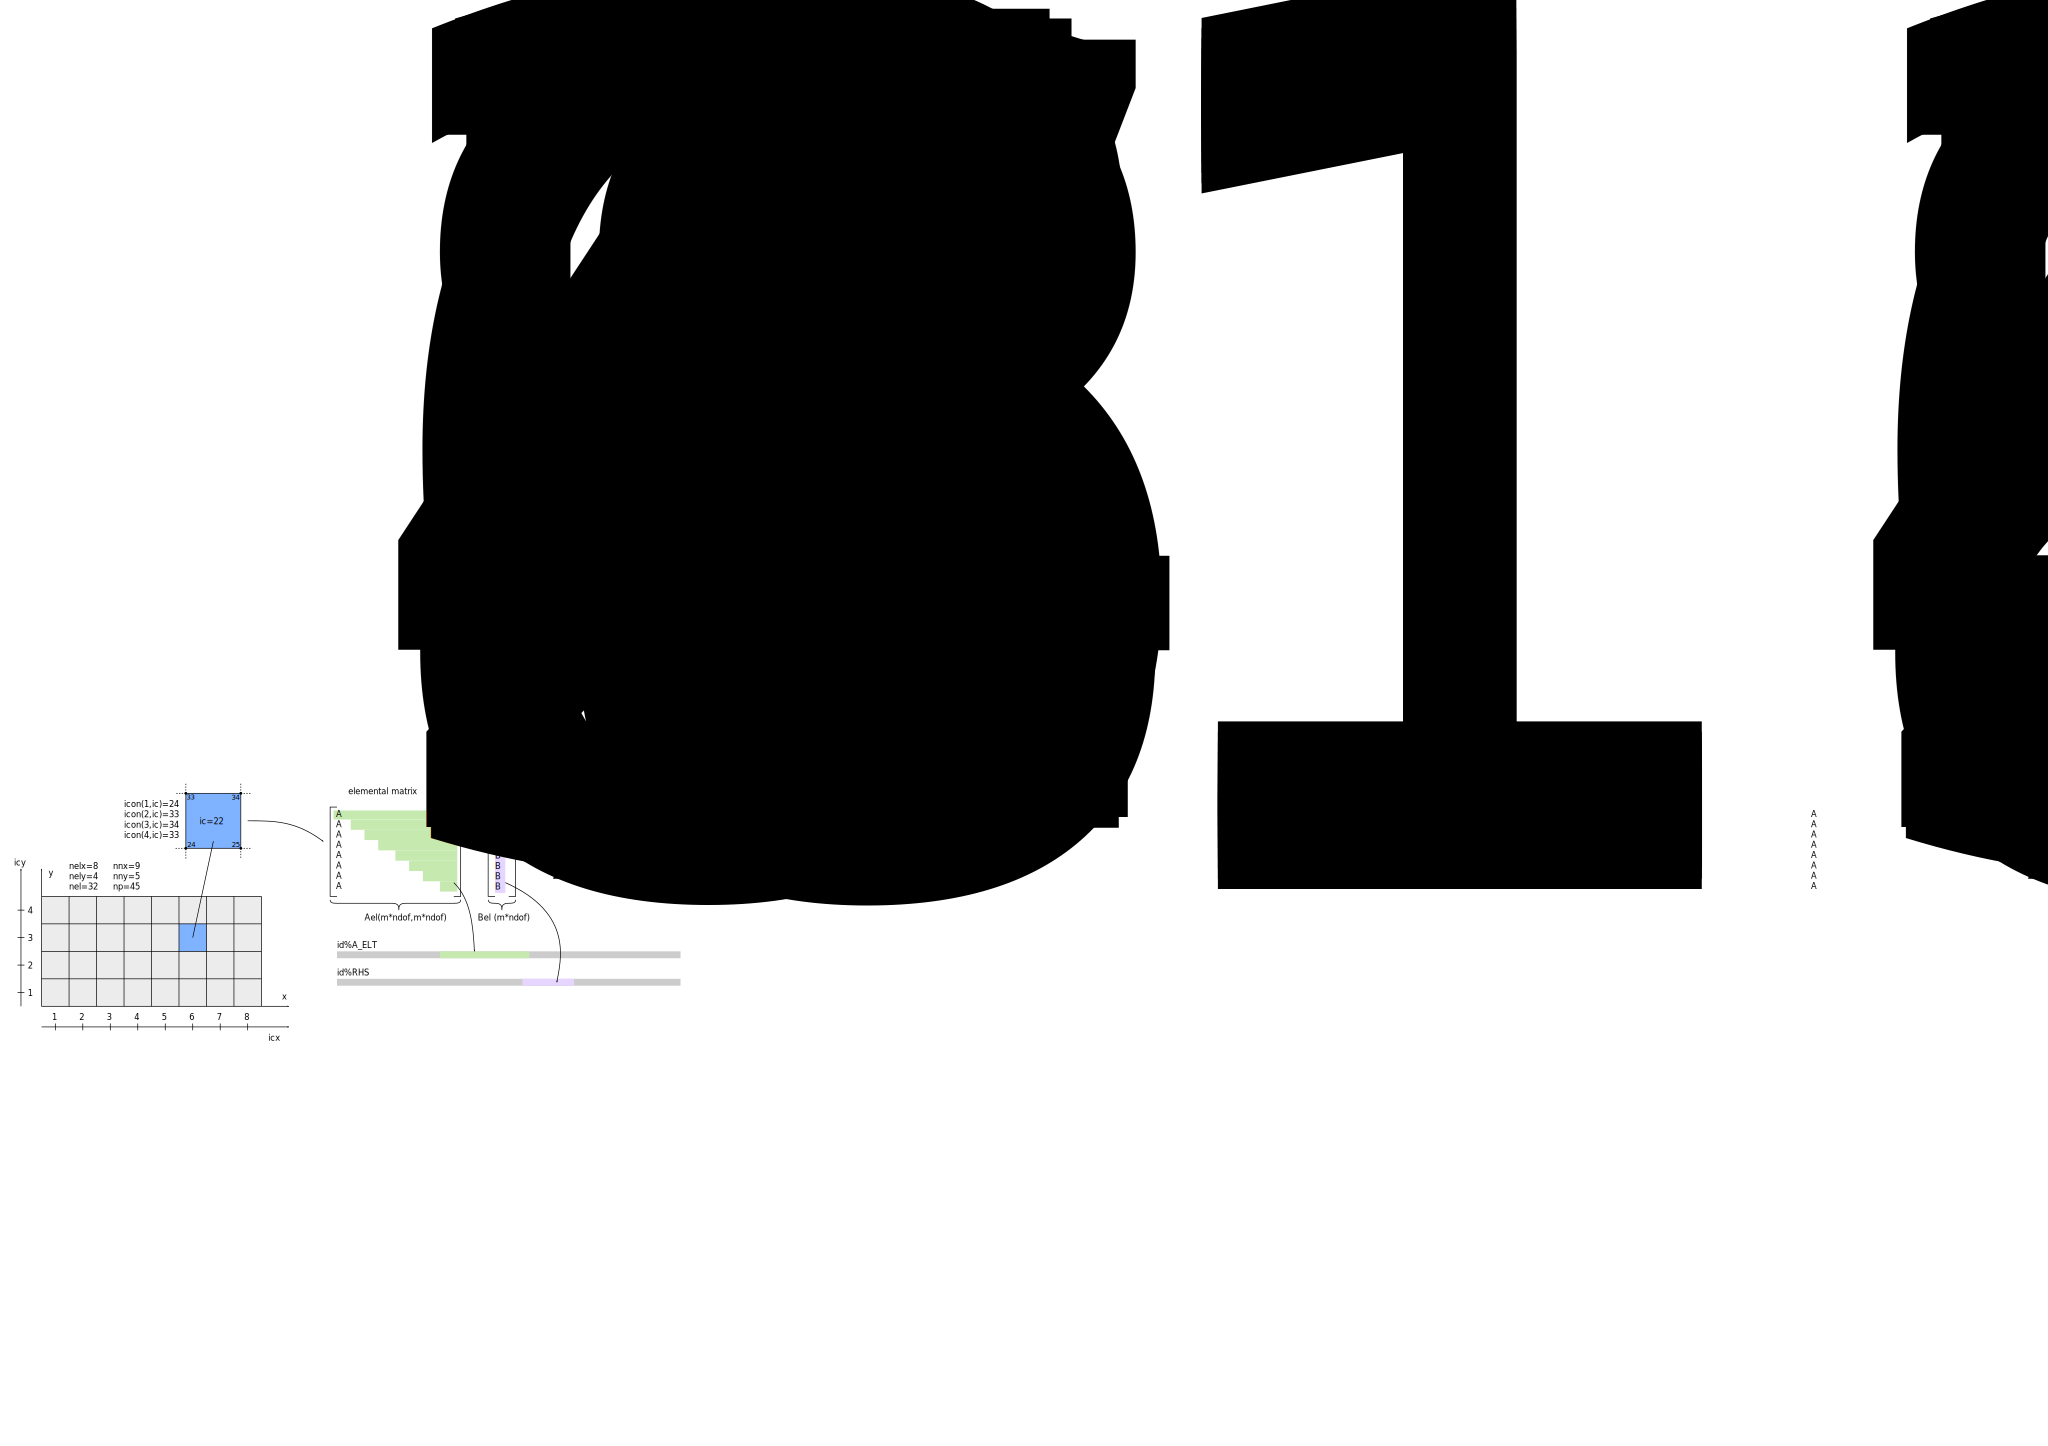
\includegraphics[width=10cm]{python_codes/fieldstone_178/images/grid}
\end{center}

The code solves the mass and momentum conservation equations first and then the heat transport equation. 
Note that there is no time integration in this work. We will be looking at a 2D domain subjected to various boundary 
conditions, material properties, buoyancy forces, ... instantaneously. In other words, there will be {\it no deformation}.



%-------------------------------------------------------------------------
\subsection*{Rheology}

In our calculations the effect of elastic deformation is neglected. Deformation is then accomodated by either viscous 
or plastic behaviour. The effective plastic viscosity is given by \cite{thie11,nabu15,spmw16}
\[
\mu_{pl} = \frac{\sigma_y}{2 \dot{\epsilon}}
\]
where $\sigma_y$ is the yield value which is a function of pressure (Drucker-Prager or Mohr-Coulomb type):
\[
\sigma_y = p \sin \phi + c \cos \phi
\]
where $\phi$ is the angle of friction, $c$ is the cohesion. 

The effective dislocation creep viscosity is given by \cite{thie11}
\[
\mu_{dl}=\frac{1}{2} f A^{-1/n} \dot{\epsilon}^{\frac{1}{n}-1} \exp \left( \frac{Q+pV}{nRT}  \right)
\]
where $A$ is the prefactor coefficient, $n$ is the nonlinear exponent, $Q$ is the activation energy, $V$ is 
the activation volume, $R$ is the gas constant. $f$ is a parameter which allows us to scale the computed 
viscosity by a given factor, as in \cite{hube11}.

In both formulae $\dot{\epsilon}$ is a scalar which stands for the square root of the 2nd invariant $E_2$ 
of the strain rate tensor (see Appendix B of \cite{thie11}):
\[
\dot{\epsilon}=\sqrt{E_2} = \sqrt{ \frac{1}{2}(\dot{\epsilon}_{xx}^2+\dot{\epsilon}_{yy}^2)+\dot{\epsilon}_{xy}^2 }
\]

In practice both viscosities are computed at each (quadrature) point of the FE mesh and the final effective viscosity 
is obtained by taking the harmonic\footnote{https://en.wikipedia.org/wiki/Harmonic\_mean} average of both values.

%----------------------------------
\subsection*{Let's run the code}

The code is available in the folder pertaining to this \stone but also 
on the GitHub platform\footnote{https://github.com/cedrict/simpleFEM\_CONTINENTALRIFT}. 
In order to download it, open a terminal (CTRL+ALT+T) and type:
\begin{verbatim}
git clone https://github.com/cedrict/simpleFEM_CONTINENTALRIFT.git
\end{verbatim}
Upon completion, make sure that the folder {\tt simpleFEM\_CONTINENTALRIFT} has been created. Bring the 
terminal prompt to the folder.
In order to compile the code, simply type:
\begin{verbatim}
make
\end{verbatim}
When/if successful, this produces the executable {\sl simplefem}.
{\color{red} note that you will need to install MUMPS\footnote{https://mumps-solver.org/index.php} first.}
Run the code by typing the following command at a terminal prompt 
\begin{verbatim}
./simplefem
\end{verbatim}

Once you have implemented the required features (see next section), the runs should last at most a few minutes. 
You will see during this time many lines appear
on your screen as the code outputs information pertaining to the calculation for every iteration.
All visualisation files are created in the OUT folder. These consist of {\sl .vtu} files (to be opened with Paraview) and {\sl .dat} ascii files. 
You need to recompile the code every single time you modify a .f90 file.

Once you are done with a particular model, simply store the files you wish to keep elsewhere on the machine and then do
\begin{verbatim}
./clean
make
\end{verbatim}


%------------------------------
\subsubsection*{Using Paraview}

In the terminal type
\begin{verbatim}
paraview &
\end{verbatim}
In OUT you will find {\sl solution\_000001.vtu}. Open it with Paraview.

[...]

%------------------------------
\subsubsection*{Using gnuplot}

Bring the prompt of the terminal to the {\tt OUT} folder. You will find in there the 
{\sl profiles.dat}, {\sl surface.dat} and {\sl convergence\_nl.dat}.
We will use gnuplot\footnote{http://www.gnuplot.info/} to plot these. In the terminal type:
\begin{verbatim}
gnuplot
\end{verbatim}
At the gnuplot terminal, type (replace 'file' by the name of the file you wish to plot)
\begin{verbatim}
plot 'file.dat' w lp 
\end{verbatim}

You can visualise multiple files at the same time as follows:
\begin{verbatim}
plot 'file1.dat' w lp, 'file2.dat' w lp, 'file3.dat' w lp , ... 
\end{verbatim}
You will find there ( http://physics.ucsc.edu/$\sim$medling/programming/gnuplot\_tutorial\_1/index.html ) 
an excellent primer on how to interactively work with gnuplot.

Scaling the data being visualised can be done as follows:
\begin{verbatim}
plot 'file.dat' u ($1/1000.):($5/1000.) w lp
\end{verbatim}
In this case it divides the values of both columns by 1000.

gnuplot can also be scripted. One advantage of such an approach is that gnuplot can then generate a pdf 
file with the figure you are interested in. You should create a file, say {\sl mygnuplot.script} which contains the following lines:
\begin{verbatim}
set term pdf enhanced
set grid
set output 'myoutput.pdf'
set xlabel 'x-axis'
set ylabel 'y-axis'
plot 'file.dat' with lp title 'opla'
\end{verbatim}

At the prompt of the terminal you can then run gnuplot as follows:
\begin{verbatim}
gnuplot mygnuplot.script
\end{verbatim}
This should have produced the myoutput.pdf file in the same folder.
You can visualise it as follows:
\begin{verbatim}
gv myoutput.pdf
\end{verbatim}

%--------------------------
\section*{Tasks ahead}

\subsection*{Basic parameters}

Basic parameters such as the domain size and the resolution are defined in {\sl simplefem.f90}.
In our case, we set $L_x$=400km and $L_y$=100km and we start with a 200x50 resolution. 

%---------------------------
\subsection*{Material layout}

We start with the spatial distribution of the four lithologies (upper and lower crusts, lithospheric mantle and seed). 
Please have a look at the setup figure of section (2) (see also \cite{nabu15} for reference). 
To begin with, the upper crust (material 1) has a thickness of 20km, the lower crust (material 2) a thickness of 10 km, 
the mantle (material 3) of 70km. The seed (material 4) is parametrised by $198km<x<202km$ and $60km<y<68km$.
Study and modify the {\sl material\_layout.f90} file in the {\tt EXPERIMENT} folder. 

%---------------------------
\subsection*{Temperature field}

We will impose a linear gradient in the crust and another linear gradient in the mantle lithosphere.
In order to do so, you will have to modify the {\sl temperature\_layout.f90} file. We fix $T=0^\circ$ at the 
surface, $T=550^\circ$ at the Moho and $T=1200^\circ$ at the bottom.

%---------------------------
\subsection*{Implementing boundary conditions}

Extensional boundary conditions are as follows: 
$-v_{ext}=-0.25$cm/yr is prescribed on the left boundary,
$+v_{ext}=+0.25$cm/yr is prescribed on the right boundary,
and the corresponding value is prescribed at the bottom so as to insure volume conservation in the domain.
Study and modify the {\sl define\_bc.f90} file.

%---------------------------
\subsection*{Implementing rheology}

Modify the {\sl material\_model.f90} file.

\begin{itemize}
\item from the strain rate components {\tt exxq,eyyq,exyq} compute the square root of its second invariant.
\item for each material, assign its $Q,n,V,A,c,\phi,\alpha,T_0$ values (see Table 1 of \cite{nabu15}). Set $f=1$ 
for all. Make sure that the cohesion for all materials is set to 20Mpa.
\item compute the effective dislocation creep viscosity {\tt mu\_dl}
\item compute the effective plastic viscosity {\tt mu\_pl}
\item compute the harmonic average {\tt mueffq} of these two quantities 
\item compute the density {\tt rhoq} as a function of temperature  
\end{itemize}


%---------------------------
\subsection*{To go further}

Hereafter is a list of tasks to be carried out. Some of the instructions are voluntarily vague so as to 
force you to think about what you are doing. For all bullet points hereunder, document your observations 
with whatever quantitative data you deem appropriate. Reminder: for each run you have a vtu file 
and various ascii files in the OUT folder. 

Relevant literature: 
Rifting \cite{hube03,hubb05,hube07,hube11,bupb09,alht11,alht12,alhf13,engl83,vacl02} 
Rheology \cite{buro11,budr08,hiko03,kawu93}

\begin{itemize}
\item Try various grid resolutions. Based on these results choose an appropriate resolution to conduct the rest of the experiments.

\item Seed size/nature. 
   \begin{itemize}
   \item Vary the size of the seed and its location. 
   \item Replace it by a temperature anomaly. 
   \item Add a second seed.
   \item Replace it by a notch in the crust-mantle lithosphere interface, i.e. the mantle intrudes in the crust at a given location over a few kms. 
   \item Replace it by a discontinuous Moho: left crust is 30 km thick while right crust is 30+X km thick
   \end{itemize}

\item Initial Temperature (Moho temperature)
   \begin{itemize}
   \item what is an acceptable range for the Moho temperature? Try the end members and document the effects these have on the system.
   \item In the presence of radiogenic heating, the steady state profile is no more linear \cite{chap86}.
   Solve steady state 1D heat transfer equation in a single layer to arrive at 
   \[
   T(y) = T_T + \frac{q_T}{k} y - \frac{H}{2k}y^2
   \]
   where $H$ is the volumetric heat production, $k$ is the heat conduction, $q$ is the heat flux at the top and 
   $T_T$ is the temperature at the top.

   In our case $H$ is taken to be $1.5\times10^{-6}$ in the upper crust and 0 elsewhere. We set $k_1=k_2=2.5$, $k_3=3.3$, and $q_T1=0.0653571$. 
   Assuming the temperature at the surface to be 0C, what is the temperature at the base of the upper crust?
   What is then the temperature at the base of the lower crust. Adjust accordingly the linear gradient in the lithospheric mantle.

%the temperature at the base of the upper crust to be 408C, and the temperature at the base of the lower crust to be 550C.
%ts1=273,ts2=681.5714,ts3=823., 
%qs2=0.035357,qs3=0.035357

\end{itemize}

\item What is the influence of the cohesion and angle of friction? 
\item The activation energy and activation volume values are obtained from laboratory measurements. What are the uncertainties on the values presented in \cite{nabu15}?
\item Boundary Conditions 
\begin{itemize}
\item what is the influence of the extensional velocity?
\item what happens when the bottom velocity is set to zero?
\item what happens when the left and right velocity values are not equal ?
\item what happens when $v_y$ is set to zero on the sides?
\item the default value for $f$ is 1. Set it to 0.01 or 100 for the lower crust.
\end{itemize}


%\item Model Geometry/ Initial Lithology

\item nonlinear convergence settings. How does the implemented nonlinear loop work? What is the effect of the tolerance value?

\end{itemize}

